\section{Explicit ODE solver}
Considering the more general case of an \textit{Initial Value Problem}.
$$
\frac{d}{d t} x(t)= \dot{x}(t)=f(t, x(t), p), \quad x\left(t_{0}\right)=x_{0},
$$
where $x \in \mathbb{R}^{n_{x}}$ and $p \in \mathbb{R}^{n_{p}}$. In the following equations, the parameters p are implicit in $f(t, x(t)) = f(t, x(t), p)$.

\subsection{Explicit Euler}
The simplest numerical solver for this problem is the Explicit Euler which discretizes the continuous ODE by taking forward steps with the $\dot{x}(t_k) = f(t, x(t))$ in each iteration $k$ \cite{JrgensenScientificEquations}:

\begin{equation}
    x_{k+1}=x_{k}+\Delta t_k f\left(t_{k}, x_{k}\right)
\end{equation}

Where $\Delta t_k$ is the step size in iteration $k$. The method is analogous to taking the tangent in $x(t_k) = x_k$ and taking a $\Delta t_k$ step along the tangent:

\begin{equation}
\frac{x\left(t_{k+1}\right)-x\left(t_{k}\right)}{\Delta t_{k}} \approx \frac{d}{d t} x\left(t_{k}\right)=f\left(t_{k}, x\left(t_{k}\right)\right)
\end{equation}

Naturally a question arises on choosing an appropriate step size $\Delta t_k$. This gives rise to Explicit Euler with fixed step size

\begin{equation*}
    \Delta t_k = \Delta t = h \quad \forall_k
\end{equation*}

And with adaptive step size where $\Delta t_k$ can change in each iteration k. The ladder approach is discussed in further detail in Section 2.3.

\subsection{MATLAB implementation fixed step size}
See the following MATLAB implementation of the Explicit Euler with fixed step size (as described in Section 2.1), well-suited for non-stiff problems.

\begin{adjustwidth*}{0cm}{-0.4cm}
\begin{lstlisting}[frame=single, language=Matlab,caption=Explicit Euler (fixed step size), label=ExplicitEulerFixie]
function [T,X, fcount] = ExplicitEulerFixedStepSize(fun,t0,tN,N,x0,varargin)
% Compute step size and allocate memory
fcount = 0;
dt = (tN-t0)/N;
nx = size(x0,1);
X = zeros(nx,N+1);
T = zeros(1,N+1);

% Eulers Explicit Method
T(:,1) = t0;
X(:,1) = x0;
for k=1:N
    fcount = fcount +1;
    [f, Jac] = feval(fun,T(k),X(:,k),varargin{:});
    T(:,k+1) = T(:,k) + dt;
    X(:,k+1) = X(:,k) + f*dt;
end

% Form a nice table for the result
T=T';
X=X';
end
\end{lstlisting}
\end{adjustwidth*}

\subsection{MATLAB implementation adaptive step size}
\label{sec:ExplicitEulerAdaptive} \label{sec:stepdoubling}
See the following MATLAB implementation of the Explicit Euler with adaptive step size, well-suited for stiff and non-stiff problems. The embedded error estimation is based on \textit{stop doubling}, i.e. estimating the error of a full step from the more accurate two half-steps. Going in greater detail with the adaptive step size:

As mentioned, an Explicit Euler is taken with step size $\Delta {t_k}$ and then two half-steps is taken with step size $\Delta t_k$ and the \textit{error} of the Euler step is estimated as difference. I.e. 

\begin{equation}
\begin{aligned}
&x_{k+1}=x_{k}+\Delta t_k f\left(t_{k}, x_{k}\right) \\
&\hat{x}_{k+1 / 2}=x_{k}+\frac{\Delta t_k}{2} f\left(t_{k}, x_{k}\right) \\
&\hat{x}_{k+1}=\hat{x}_{k+1 / 2}+\frac{\Delta t_k}{2} f\left(t_{k}+\frac{\Delta t_k}{2}, \hat{x}_{k+1 / 2}\right) \\
&e_{k+1}=\hat{x}_{k+1}-x_{k+1}
\end{aligned}
\end{equation}

The r-coefficient is then calculated relative to chosen tolerances of the solution

\begin{equation}
r_{k+1}=\max _{i \in\{1, \ldots, n\}}\left\{\frac{\left|\left(e_{k+1}\right)_{i}\right|}{\max \left\{\text { abstol },\left|\left(x_{k+1}\right)_{i}\right| \text { reltol }\right\}}\right\}
\end{equation}

All cases where $r_{k+1} > 1$ is then rejected such that the error in each step $e_{k+1}$ is never great than the abstol nor the relative tolerence (reltol) times $(x_{k+1})_i$. 
\\
If $r_{k+1} > 1$ the step size is decreased until the criteria is fulfilled. Similarly, if $r_{k+1}$ is very low, i.e. the error is very low compared to our tolerances, the step size should be increased.
The step size $\Delta t_{k+1}$ is increased or decreased with the formula

\begin{equation}
\Delta t_{k+1}=\left(\frac{\varepsilon}{r_{k+1}}\right)^{1 / 2} \Delta t_{k}
\end{equation}

Where $\epsilon$ represents a target $r_{k+1}$ value. For robustness, a minimum and maximum scaling factor of the step size is chosen and denoted \textit{facmin} and \textit{facmax}. See the MATLAB implementation below for the Adaptive Explicit Euler. Note that $h = \Delta t_{k}$ has been used.

\begin{adjustwidth*}{0cm}{-0.4cm}
\begin{lstlisting}[frame=single, language=Matlab,caption=Explicit Euler (adaptive step size), label=ExplicitEulerFixie]
function [T,X,fcount,nreject] = ExplicitEulerAdaptiveStep(...
    fun,tspan,x0,h0,abstol,reltol,varargin)
epstol = 0.8;
facmin = 0.1;
facmax = 5.0;

t0 = tspan(1);
tf = tspan(2);
fcount = 0;
nreject = 0;

% Initial condtions
t = t0;
h = h0;
x = x0;

% Output
T = t;
X = x';
%% Main algorithm
while t < tf
    if (t + h >tf)
        h = tf-t;
    end
    fcount = fcount+1;
    f = feval(fun,t,x,varargin{:});

    AcceptStep = false;
    while ~AcceptStep
        %Take step of size h
        x1 = x+h*f;

        %Take step of size h/2
        hm = 0.5*h;
        tm = t + hm;
        xm = x + hm*f;
        fcount = fcount +1;
        fm = feval(fun,tm,xm,varargin{:});
        x1hat = xm + hm*fm;

        % Error estimation
        e = x1hat-x1; % Estimate of global error
        r = max(abs(e) ./ max(abstol,abs(x1hat).*reltol));

        AcceptStep = (r <= 1.0);
        if AcceptStep
            t = t+h;
            x = x1hat;

            T = [T;t];
            X = [X;x'];
        else
            nreject = nreject+1;
        end
        % Asymptotic step size controller
        h = max(facmin, min(sqrt(epstol/r), facmax))*h;
    end
end
\end{lstlisting}
\end{adjustwidth*}

\subsection{Van der Pol}
The Van der Pol oscillator problem is used extensively throughout this report to compare the different numerical solvers. It is defined as the 2nd order differential equation

\begin{equation}
\ddot{y}(t)=\mu\left(1-y(t)^{2}\right) \dot{y}(t)-y(t)
\end{equation}

Which can be rewritten to a 1st order differential equation \cite{JrgensenScientificEquationse}: 

\begin{equation}
\label{eq:vanderpol}
\begin{aligned}
&\dot{x}_{1}(t)=x_{2}(t) \\
&\dot{x}_{2}(t)=\mu\left(1-x_{1}(t)^{2}\right) x_{2}(t)-x_{1}(t)
\end{aligned}
\end{equation}

Where $y(t) = x_{1}(t)$.


\\\

The phase potraits as obtained by solving the Van der Pol problem (Eq. \ref{eq:vanderpol}) using the Adaptive Explicit Euler and Fixed (step size) Explicit Euler is seen in Figure \ref{fig:2_4a} and \ref{fig:2_4b}. The problem is solved for t = [0, 32] with $\mu = 3$ and $\mu =20$. Tolerances chosen are $reltol = abstol = \{10^{-2}, 10^{-4}, 10^{-6}\}$. Now a natural question arises, which fixed step sizes $h$ should be chosen for comparison with the adaptive method? The fixed step size $h$ was chosen to result in same number of steps as for the adaptive solution for comparison purposes.

\\
Clearly, for the stiff problem ($\mu = 20$) the fixed step size $h \approx 0.1$ is infeasible. The method is unstable and explodes towards $\infty$ (Figure \ref{fig:2_4a}). For the non-stiff problem ($\mu = 3$), the $h \approx 0.1$ is biased compared to the adaptive methods.
\\

When looking at tolerances of $\{10^{-4}, 10^{-6}\}$ seen in Figure \ref{fig:2_4b} the fixed step size is a lot more accurate, albeit a small bias in the non-stiff problem. For the stiff-problem $h=\frac{1612}{32}$ is very biased and only slightly biased for $h=\frac{14411}{32}$. There is no distinguishable difference between the Adaptive Euler and ode45/ode15s for tolerances $\geq 10^{-4}$.
\\

Note however that the Adaptive Explicit Euler uses a lot more function evaluations than the Fixed Explicit Euler. The choice is a trade-off between speed and accuracy.

\begin{figure}
    \centering
    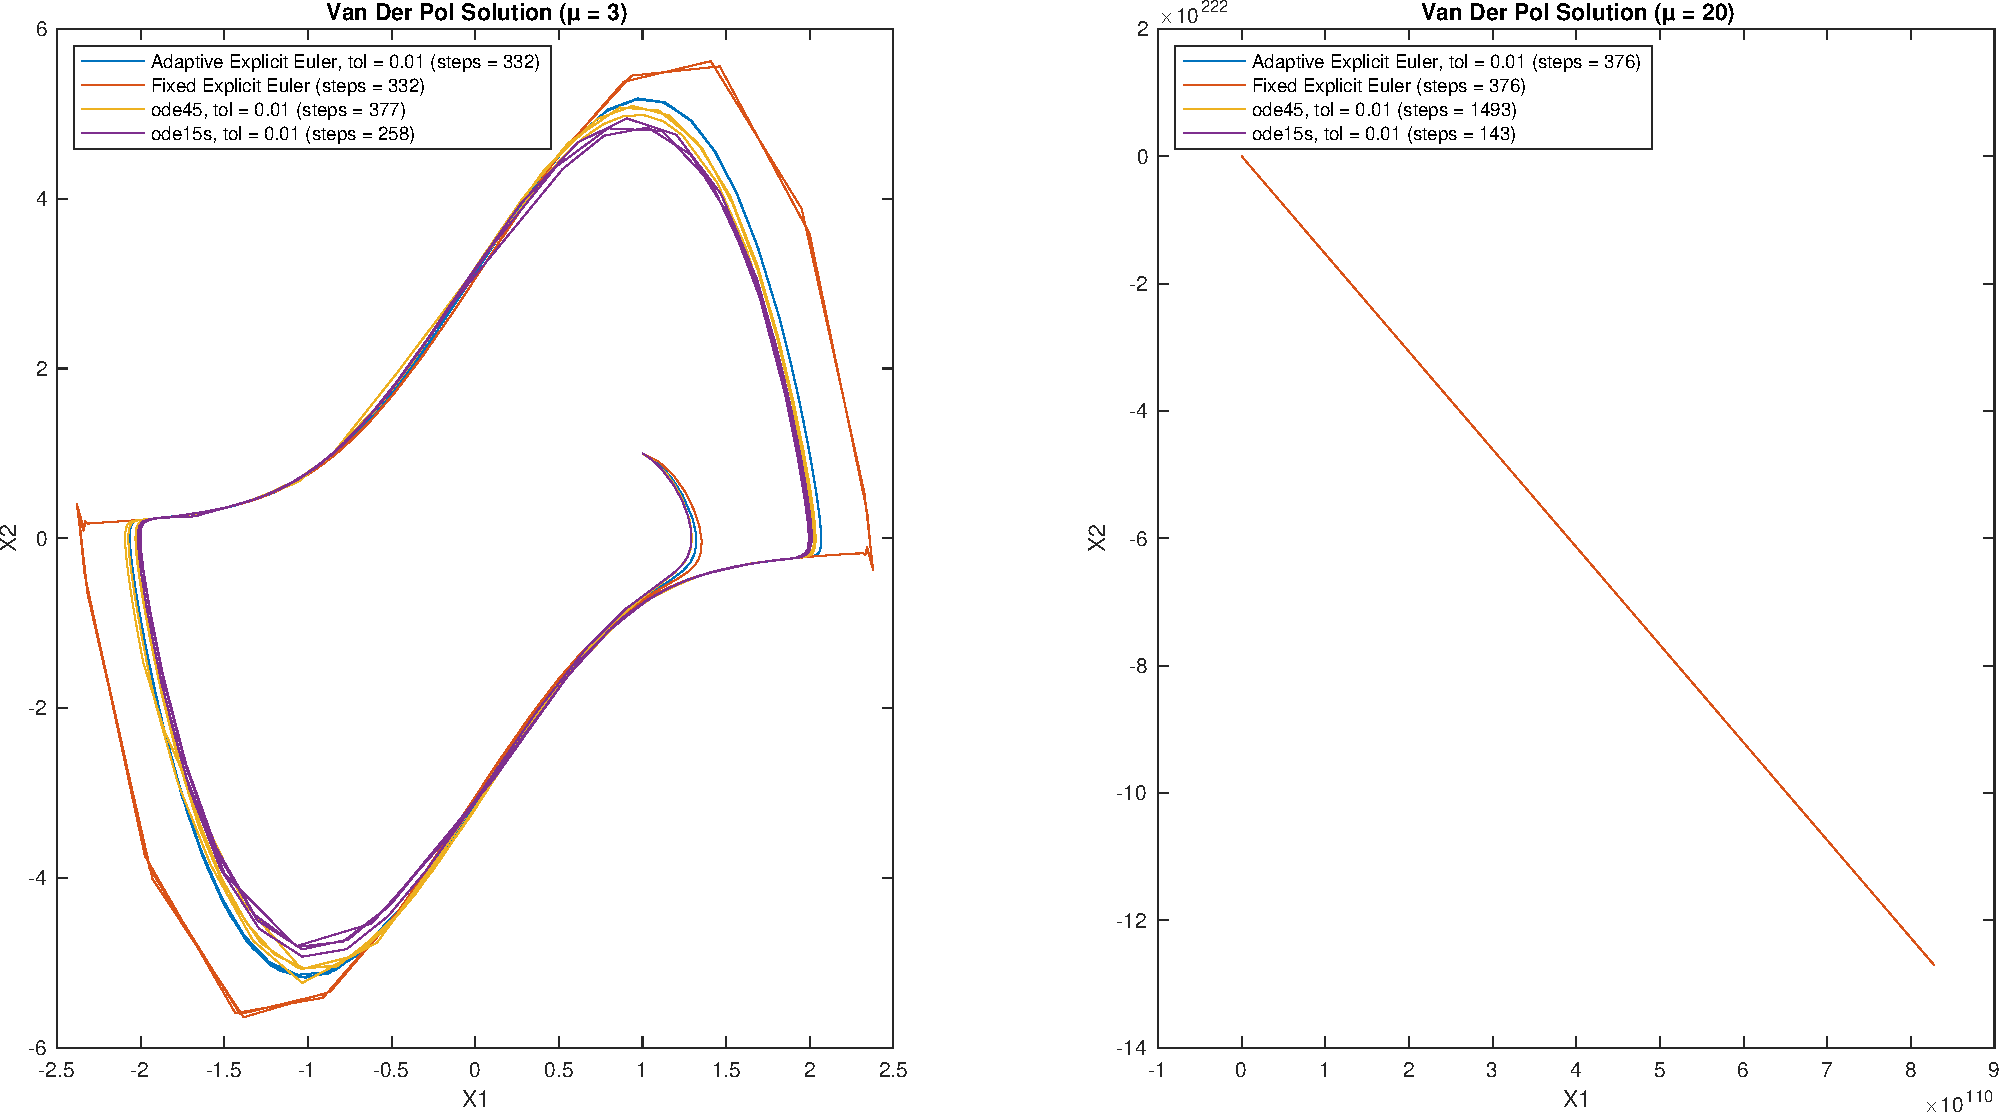
\includegraphics[width=\textwidth]{plots/2_4main_02.pdf}
    \caption{Explicit Euler method tested on the Van der Pol problem. Both an adaptive step size strategy with tolerance = 0.01 and a fixed step size strategy fixed to equal number of steps is applied.}
    \label{fig:2_4a}
\end{figure}

\begin{figure}
    \centering
    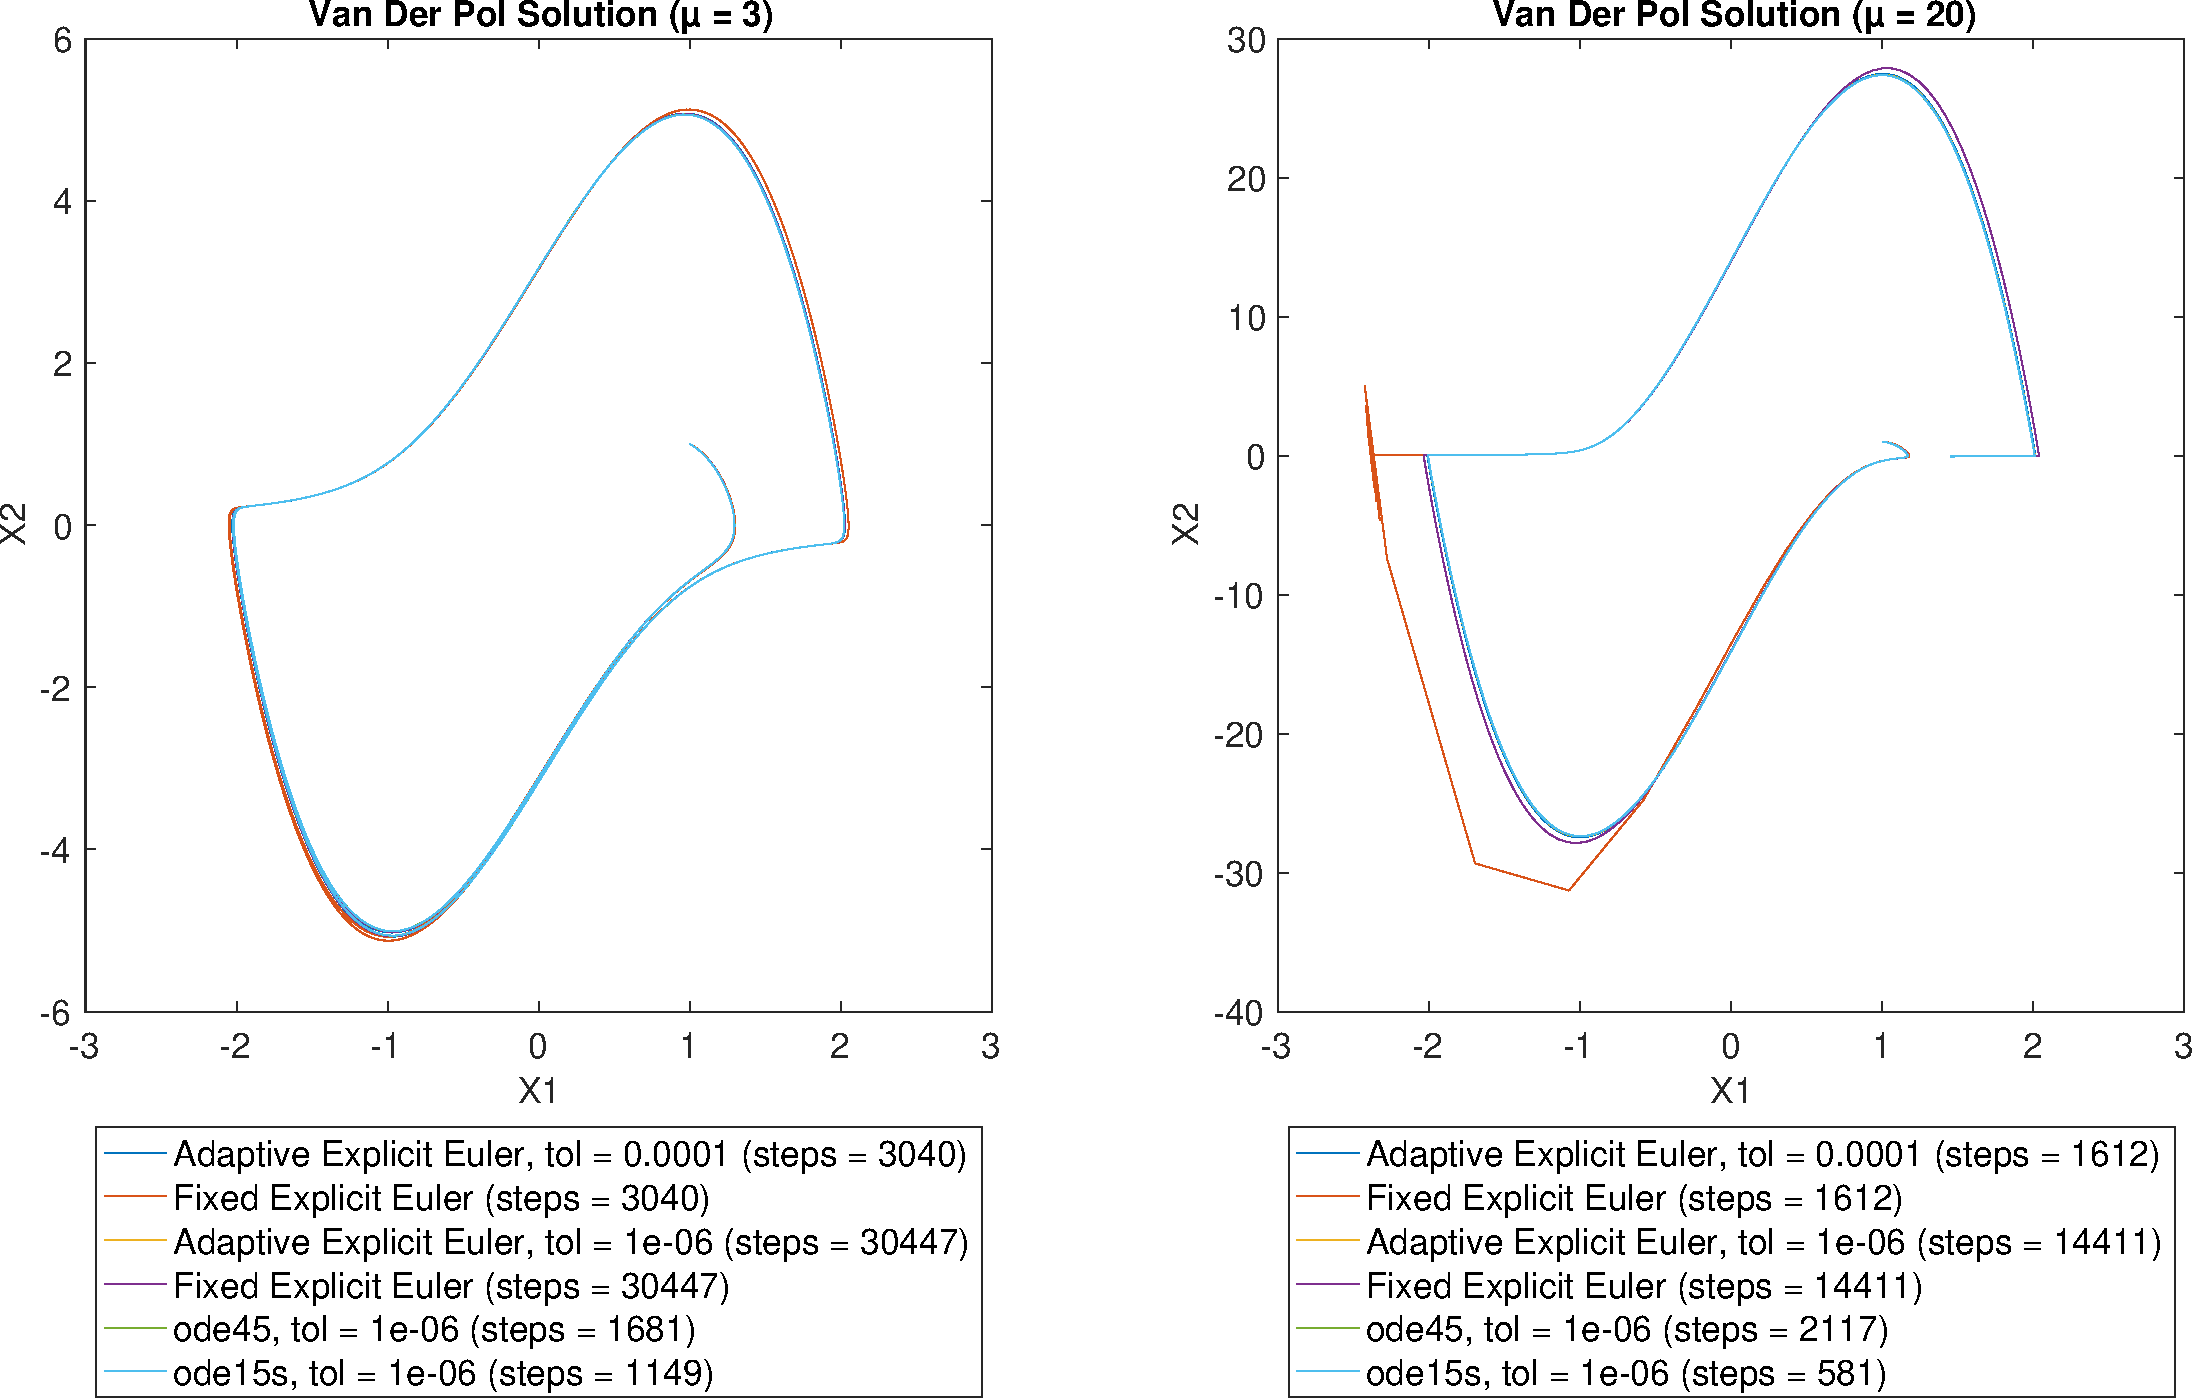
\includegraphics[width=\textwidth]{plots/2_4main_04_06.pdf}
    \caption{Explicit Euler method tested on the Van der Pol problem. Both an adaptive step size strategy with tolerances $\in \{10^{-4}, 10^{-6}\}$ and a fixed step size strategy with an equivalent number of steps is applied.}
    \label{fig:2_4b}
\end{figure}

\subsection{Discussion of interface}
The methods have been implemented in a similar fashion to MATLAB's ode45 and ode15s for comparison purposes. For better comparison of fixed vs. adaptive step size, the implementation of the fixed step size was designed to be able to take a $N$ number of steps as input.